%!TEX root = /Users/smsohan/Taggy/Thesis/ucalgthes1_root_0.tex
\fancyhead[RO,LE]{\thepage}
\fancyfoot{} 
\chapter{Introduction}
In this thesis I have presented a machine learning based technique to build an organic knowledge center for distributed agile teams. The knowledge is captured from emails and instant messages and automatically tagged to the relevant project requirements or user stories. I have discussed about a prototype implementation of the technique named Taggy. Taggy has correctly found the relevant user story for ~76\% of 4,745 emails from 9 agile project teams. I have also conducted a user study and found encouraging feedback about the technique and its implementation. In a nutshell, this thesis documents the details of my auto-tagging technique, its novelty compared to some of the existing solutions, a prototype implementation and the evaluation results based on real-world data as well as it's qualitative feedbacks.

The process of agile software engineering is a collaborative approach which incrementally delivers software in small iterations, preferably of two to four weeks. Agile teams commonly use ``user stories'', a small description of a desired feature in everyday language, to capture the software's requirements. An example user story is as follows:\\
\begin{quote}
As a shopper, I want to pay online to checkout my shopping cart using MasterCard, Visa or Amex credit card from a secured web page only.
\end{quote}
The details of such user stories are discussed on an ongoing basis among the people involved in a project. For example, as the engineering team starts working on the stories, they often consult with customers and other teammates to further clarify such user stories. Whenever possible, face-to-face communication is preferred as the principal communication medium between customers and developers in agile processes \cite{am, xp, scrum, xp_up}. In collocated setups, where the team members work in close proximity, such informal communication relays the tacit knowledge among the people. 

However, for distributed projects, especially when there is a huge time zone difference among people, face-to-face communication becomes infeasible. To mitigate this difficulties in communication, people use alternatives such as phone calls, emails, instant messaging, wikis, web forums and so on. So, in such setups communication is often text based instead of oral and direct knowledge sharing. In this sense, distribution makes it easy to capture the knowledge about the user stories since much of it is textual and electronic. For an example, considering the aforementioned user story, the developer may send the following email to the customer to further clarify expectations.\\

\begin{quote}
\textbf{Subject:} Clarification required on online credit card payment\\
\textbf{Hi Bob:}\\
Please clarify if the shoppers need to provide the security code of the credit card while doing checkout.
\end{quote}

Since email is a persistent tool in the sense that they remain in the inbox unless deleted, one can use this knowledge in future. But, email is also a personal tool and it is hard to transfer a selection of project related emails from the email inbox in a reusable format. The same is true for instant messages as well. So, when someone leaves the team, it becomes hard to access that knowledge if needed later down the road. To retain this useful information, this thesis explored a machine learning based technique. As a proof of concept, the technique is also implemented and evaluated through a prototypical tool called \textbf{``Taggy''} that automatically grabs and tags the emails and instant messages with relevant user stories.

The relationship between a user story and email or instant message is not explicit. To establish the implicit relation, Taggy uses  Case Based Reasoning (CBR). For auto-tagging, a CBR system is designed to look at the text, people, and temporal similarity between emails and user stories. The evaluation results show that a well trained software such as Taggy can auto-tag emails with user stories. Also, we found that combining contextual information with text similarity helps to find the related user stories with higher accuracy than using just text match alone.

In the existing literature, attempts have been made to capture software project related knowledge following several alternative approaches. For example, commercial tools exist that link software code commit messages with a requirement or ticket given the ticket number is present inside the commit log. Also, another approach is to use wiki or online message threads, where the contents are manually linked with the user stories. However, to use such approaches, one needs to remember identifiable tokens or learn markup syntax (e.g. wiki), which is often burdensome for business users. To reduce this learning curve and effort required of human users, Taggy builds a knowledge base by automatically tagging emails and instant messages with user stories. 

The remaining part of this chapter is organized as follows: First, I discuss the necessary background material about user stories and distributed agile projects to develop an understanding of the terms used in this thesis; then, the research motivation is discussed; finally, I present the research goals and related challenges.

%Start the body text
\section{User Stories - An Overview}
In agile projects, user stories are used to capture requirements. In short, user stories represent the need for a feature from the view point of a potential user of an application. Cohn \cite{user_stories_applied} defines user stories as follows:\\

\begin{quote}
	A user story describes functionality that will be valuable to either a user or purchaser of a system or software. User stories are composed of three aspects:
	\begin{itemize}
		\item a written description of the story used for planning and as a reminder
		\item conversations about the story that serve to flesh out the details of the story
		\item tests that convey and document details that can be used to determine when a story is complete
	\end{itemize}
\end{quote}

As outlined in the above definition, conversation plays a central role in fleshing out the details of user stories. Jeffries \cite{ron_jeffries} and Davies\cite{rachel_davies} also emphasize the role of conversation as a key component of user stories.

Wake, author of \cite{bill_wake}, suggested a popular acronym, INVEST, that defines good stories being Independent, Negotiable, Valuable to users, Estimable, Small and Testable. However, to hold all these characteristics while remaining Small essentially points to conversation as means of detailing the user stories.

In an agile project, the customer or a representative of the customer is responsible for coming up with these user stories with the help of the stakeholders. Next, the user stories are prioritized in a list known as ``Product Backlog''. At the start of every iteration (typically two to four weeks), the team picks the top user stories from the product backlog to create an ``Iteration Backlog'' with the target to deliver the functionality for each of these user stories at the end of the iteration. A user story is supposed to be limited in scope so that it can be delivered within a single iteration. However, the details about the user stories are laid out on an ongoing basis during the iteration through customer collaboration and feedback.

One or more team members are assigned to deliver a user story, which may involve design, development, testing and such tasks. It is a common practice that the customer and the assigned team members collaborate to fine tune the user story details. Collocated teams often use sticky pads on a team wall or whiteboard to visualize the iteration backlog and track progress. Figure~\ref{fig:scrum_wall} shows a ``Scrum Wall'', where user stories are grouped based on their development status.

\begin{figure*}[bt]
	\centering
	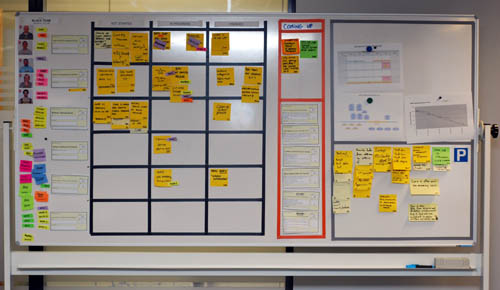
\includegraphics[width=\textwidth]{ScrumWall.jpg}
    \caption{A Scrum Wall. Source: http://www.xqa.com.ar}
	\label{fig:scrum_wall}
\end{figure*}

However, distributed agile teams often use a virtual team walls in place of a physical wall so that it is usable across several geographical locations. Figure~\ref{fig:target_process_wall} shows such a virtual wall taken from ScrumPad.

\begin{figure*}[bt]
	\centering
	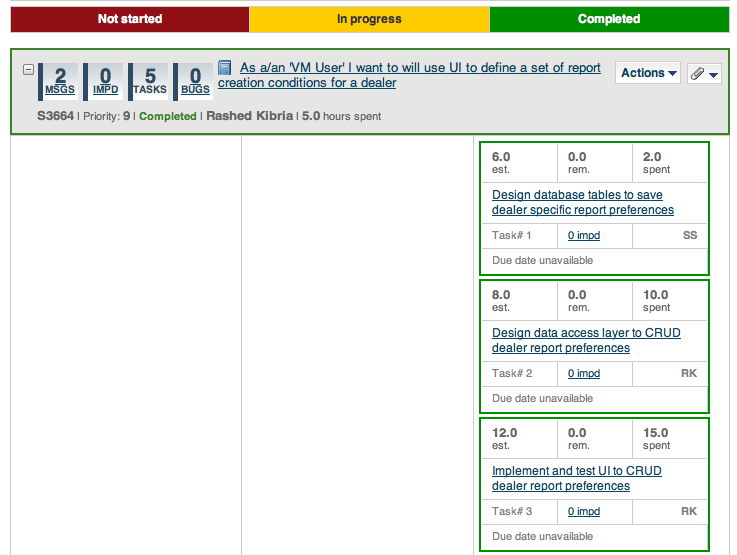
\includegraphics[width=\textwidth]{ScrumPadWall.png}
    \caption{A Virtual Scrum Wall. Source: http://www.scrumpad.com}
	\label{fig:target_process_wall}
\end{figure*}


\section{Distributed Agile Projects}
The members of a distributed agile project work from different geographical locations using agile principles. In practice, the distribution can take several models such as the following three outlined by Braithwaite et al \cite{xp_expanded}:

\begin{quote}
\begin{enumerate}
	\item Agile outsourcing - the development team is offshore to the customer.
	\item Agile dispersed development - developers are spread over different locations, such as open source projects.
	\item Distributed agile development - customers are distributed and one development team is distributed evenly so that each customer has a part of the team to closely work with.
\end{enumerate}
\end{quote}

Again, the geographical distribution can be as near as office across the road or as far as the opposite side of the world. For example, a team may work for a customer within the same city or a country separated by ten hours of time zone difference. Distributed agile teams often use different electronic communication channels such as emails, instant messaging, wikis, forums and online project management tools to uncover important details about the user stories. Scrum and XP are two popular agile specifications \cite{scrum, xp}.

\begin{figure*}[bt]
	\centering
	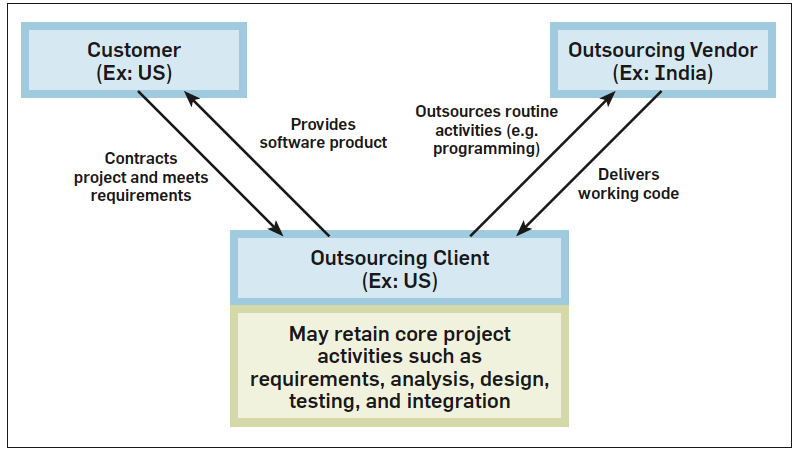
\includegraphics[width=\textwidth]{Distributed.png}
    \caption{An Example Agile Outsourcing Model. Source: \cite{modified_agile}}
	\label{fig:distributed}
\end{figure*}

Figure~\ref{fig:distributed} shows an example of an outsourced agile project taken from \cite{modified_agile}. As seen in this example, a distributed agile project may employ people working on different roles across the globe.

Cost savings has been identified as one of the principal deciding factors for distributing projects across the globe \cite{practical_considerations}. However, projects also go distributed to utilize global talent supply and local knowledge \cite{fully_distributed, modified_agile}. Previous studies have reported success with distributed agile projects. For example, Sutherland et al. reported a linear scalability with a globally distributed outsourced team following a Fully Distributed Scrum model \cite{fully_distributed}. Similarly, Yahoo! had success with distributed teams that valued people over process and exercised the right information sharing formats and timing \cite{yahoo}.

To ensure a shared view of the ``Product Backlog'' and ``Iteration Backlog'', distributed teams often use web-based project management tools. There are a number of such tools available commercially such as ScrumPad, VersionOne etc. as well as open-source \cite{scrum_pad, version_one} such as XPLanner, Trac etc.\cite{xplanner, trac} Such tools help people working remotely to have a single backlog around which to collaborate. 

\section{Research Motivation}
The existing literature about collaboration in distributed agile software projects suggests the use of various electronic mediums to compensate for missing face-to-face communication. Because of time zone differences, such teams often use asynchronous communication tools such as email and wikis in addition to synchronous ones such as telephone calls, instant messaging, etc. For example, Robarts \cite{practical_considerations} found that teams would follow up with a written email after they had a telephone meeting to ensure the discussion was clearly understood. Moreover, of all the available written communication tools, email has been regarded as the most-widely used by several former studies \cite{collaboration_in, on_coord}. Additionally, even in collocated settings, people often use emails to communicate as it doesn't require an immediate response from the recipient or the overheads of scheduled meeting.

Although having multiple communication channels adds flexibility to collaboration, it also means that knowledge gets fragmented across different channels. This fragmented knowledge may be spread over the project management tool, wiki, emails, instant messages and other places. Basili et al. provided the following list of experiences related to the lack of access to available information \cite{implementing_an_experience}:

\begin{quote}
\begin{itemize}
	\item An employee left with short notice. The organization lost all of its experience in a certain area and tries to recover it, but it doesn't even know what experience was lost.
	
	\item A consultant spends three weeks developing a course that already exists because he doesn't know that it was done before.
	\item Someone repeats a \$35,000 mistake for which there is a simple solution.
	\item A consultant gave a customer a promise, but is now busy with other work. No one else knows about his promise so it doesn't happen.
	\item An employee learned a lot during a project, but has no time for packaging and dissemination so the knowledge cannot be leveraged.
	\item A new employee is hired, but is for a long time considered a burden instead of help because he needs detailed support from his coworkers, who do not have sufficient time to help him.
	\item (continued...)
\end{itemize}                               
\end{quote}


For agile teams, this situation can be improved with a useful knowledge management solution. To retain the important details about the user stories, one needs to combine these fragmented pieces into a centralized repository. But looking into email inboxes of colleagues to do this may violate their privacy, if it is even available in the first place. Even worse, when a teammate leaves, her emails are lost as well. So, the fragmented pieces of knowledge is either lost or very hard to combine together. Even if one has access to the emails, manually copy-pasting all the emails and tagging them with the relevant user stories would be a time consuming task. The following user story and email collaboration shows an example of knowledge fragmentation:

\begin{quote}
	\textbf{Available in Project Management Tool}\\
	\textbf{User Story}\\
	\textbf{Title:} ``As a/an VM System I want to load Auction data from NADA data file''\\
	\textbf{Description:} Please see the 3 documents related to Auction data
	\begin{enumerate}
		\item Auc Layout
		\item \textbf{Regions Table}
		\item AucData.zip
	\end{enumerate}
\end{quote}

In this example, the user story represents data integration with a company named NADA. NADA provides vehicle auction information for regions denoted by a ``region code''. However, as the developer starts working on NADA integration, she asks the following question about the region code to the customer through email. 

\begin{quote}
\textbf{Email\#1 (From Developer to Customer)}\\
\textbf{Subject:} ``Initial Questions regarding NADA region value''\\
\textbf{Body:} We found that the Region value can be \textbf{Alpha-numeric} that will be received from NADA Auction. But, the NADA WS accepts only \textbf{Numeric} Region value. Is there any conversion rule to convert the region value into numeric? \\
Thanks
\end{quote}

To answer this question, the customer replies with the following email.

\begin{quote}
\textbf{Email\#2 (From Customer to Developer)}\\
\textbf{Subject:} ``RE: Initial Questions regarding NADA region value''\\
\textbf{Body:} I talked to NADA and they provided me with the \textbf{attached conversion table} for \textbf{Alpha-numeric} to \textbf{Numeric} region codes.
\end{quote}

Please note that the email from the customer included a conversion table for ``region codes''. 

Given this example, if some of the team members only look at the user story, they will find partial information about it. So, the whole conversion of ``region code''  may be confusing to them. However, when they can see the emails along with the user story, they may have a better understanding about this user story.

This information may be required since a distributed agile team have to cope up with changes in team composition as new people will join and some people may leave. So, if it is possible to combine the fragmented knowledge from different places such as emails, instant messages and project management tools, one can find the important details of the user stories. Such details may not be obvious when only the user story is available. Similarly, the knowledge can help in testing of the features since it is expected to contain customer feedbacks and clarifications on user stories.

The motivation for this thesis stems from the pursuit of developing an agile knowledge base by combining the fragmented knowledge from emails, instant messages and project management tools with the least possible human efforts.

\section{Research Problem}
In software development projects, developers sometimes leave the team for various reasons. As said before, in distributed agile projects, important knowledge is often shared by emails. To transfer this knowledge for future use, one first needs to find the project related emails. Secondly, in such setups people often use web-based project management tools to capture user stories and planning information. If the emails can be related to specific user stories in the project management tools, then another developer on the team will be able to easily find the necessary information about a user story when required.

From a team member's point of view, manually finding and relating the emails with user stories is a time-consuming and costly process. This essentially means copying the emails from an inbox and putting them into a system and linking with a user story. This manual process is cumbersome and time consuming. However, if an application can do this automatically, then it may work as a knowledge-base even after someone leaves the team. Such an application needs to be unobtrusive so that it doesn't require much human effort. So, a technical solution needs to be in place that can capture the project-related communication without violating people's privacy. For example, it cannot look into the email inbox of a developer nor should it ask developers to manually enter their chat logs into the system.  

The core technical challenge in devising such a software system is understanding the emails and relating them to specific user stories. The relation between an email and a user story is not explicit. Alternative approaches to make it explicit, such as using identifiable tokens in email subjects, also makes the communication process obtrusive as it adds an extra step to lookup the proper token or memorizing it before writing an email. To alleviate this extra step, one can modify email clients to do the lookup. But doing so for the multitude of email clients including the ones on mobile phones is cumbersome. Also, it imposes a behavioral change or a learning curve for the people at the business end.

To find out the implicit relation between a free-format email and a use story, an application needs to handle similarity between two texts, which is a standard problem. Moreover, emails may not show very high text similarity with the related user stories. This text component makes the relevance between a user story and an email an approximation or fuzzy match. Also, pure text retrieval limits how accurate the assignment of email and user stories can be. This is because people use different vocabulary and often a tacit communication exists underneath a written communication. Using context information has the potential to increase this accuracy of user story-email matching. So, a software system needs to be able to combine both the text and context similarity to auto-tag emails with user stories.

To account for the context, one needs to use the associated meta information that is available. The context of an email and a user story are not the same. For example, the context of an email has a time-stamp, sender, recipients and past conversations. On the other hand, user stories have a different context, such as their development time or iteration timeframe, developers and customers. An auto-tagging solution needs to use these contextual details meaningfully so that each component gets an appropriate weighting in the relevance computation. So, it is important to have a formula that produces a similarity ranking which considers both the fuzzy text similarity and the associated context relevance.

The technical challenge is to evaluate the accuracy of the auto-tagging system. For the auto-tagging to be useful, it shouldn't make too many mistakes in finding similarity. The accuracy of this system needs to be tested using real-world data. 

Another technical challenge is to design an adaptive auto-tagging system so that it can adapt to different communication patterns. Since distributed agile teams across the world have differences in who, how and when they communicate about their user stories, the auto-tagging system needs to adjust its similarity computation accordingly. For example, one team might spend more time communicating about user stories that are currently under development while another team might prefer to discuss about the upcoming ones. An auto-tagging system that uses the meta information of time needs to learn this pattern to make a right decision.


\section{Research Goals}
The principal goal of this research is to develop a technique to automatically read and relate emails and instant messages with user stories based on agile project context. A proof of concept tool implementation is required to test the technique. The tool needs to minimize human efforts in doing so. Another complementary goal is to evaluate the tool using real world data. The technique and its prototypical implementation are discussed in Chapters ~\ref{ch:taggy}. The evaluation of the tool is presented in Chapter~\ref{ch:evaluation}.

\begin{figure*}[h!]
	\centering
	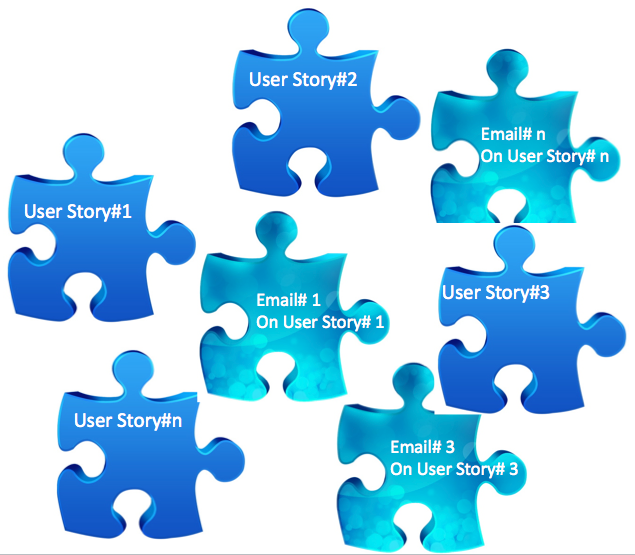
\includegraphics[width=\textwidth]{Jigsaw.jpg}
    \caption{Jigsaw Puzzle Visualizing the Auto-Tagging Problem}
	\label{fig:jigsaw}
\end{figure*}


Figure~\ref{fig:jigsaw} visualizes the research goal as it shows the fragmented knowledge from project management tools and email inboxes to be combined in a jigsaw puzzle. The target is to automatically solve this puzzle so that each user story is surrounded by it's related emails and vice versa.

This research also aimed to investigate the difficulties involved in solving the various aspects of the research problem, namely i) relevance ranking of user stories for a given email, ii) using text similarity in addition to context relevance, iii) evaluating auto-tagging accuracy and iv) developing an adaptive auto-tagger. The findings from this investigation are expected to provide a foundation for next level of research in this area.

\section{Key Contributions}
Results from this research have been published and presented at XP 2010 \cite{auto_tagging}. 

The key contribution of this research is that it demonstrates a novel approach to building a knowledge-base for distributed agile teams from emails, instant messages and user stories. This approach has a similar motivation to that found in some previous work, such as clustering email archives\cite{using_hybrid}, tagging forum messages with source code change set\cite{hipikat, hipikat_2} and using wikis to share knowledge. However, this research shows a machine learning approach to conglomerate fragmented knowledge from emails, instant messages and project management tools which minimizes human efforts.
                                  
Another key contribution is that it shows that text and context similarity can be used to find relevance between two different types of entities such as emails and user stories, where the degree of text similarity may be inadequate. I have used Case Based Reasoning (CBR) for auto-tagging. Similar to this auto-tagging solution, other CBR systems concerning different entities may also utilize this technique.
